\documentclass{beamer}
\usetheme{metropolis}           % Use metropolis theme
\usepackage{appendixnumberbeamer}
\usepackage{epigraph}
\usepackage{color}
\usepackage{amsopn}
\usepackage{tabto}

%%% Bibliography
\usepackage[backend=bibtex, style=authoryear]{biblatex}
\AtBeginBibliography{\tiny}
\bibliography{../bibliography.bib}

\setbeamercolor{background canvas}{bg=white}
\setbeamercolor{title}{fg=gray!60}
\setbeamercolor{subtitle}{fg=gray!20}
\setbeamercolor{author}{fg=gray!60}
\setbeamercolor{institute}{fg=gray!20}

\newcommand{\todo}{\alert{TODO}}
\newcommand{\itemBullet}{\scriptsize$\blacksquare$}
\setbeamertemplate{itemize item}{\itemBullet}
\setbeamertemplate{itemize subitem}{\itemBullet}
\setbeamertemplate{itemize subsubitem}{\itemBullet}
\newcommand{\E}{\mathop{\mathbb{E}}}
\DeclareMathOperator*{\argmax}{arg\,max}
\newcommand{\epiParSpace}{\vskip 1.5ex}
\newcommand{\p}{\mathbf{p}}

\title{Dynamic Routing Between Capsules}
\subtitle{by S. Sabour, N. Frosst and G. Hinton (NIPS 2017)}
\author{presented by Karel Ha}
\institute{Pattern Recognition and Computer Vision Reading Group}
\date{27\textsuperscript{th} March 2018}                         % no dates

\begin{document}
  {
    \usebackgroundtemplate{
      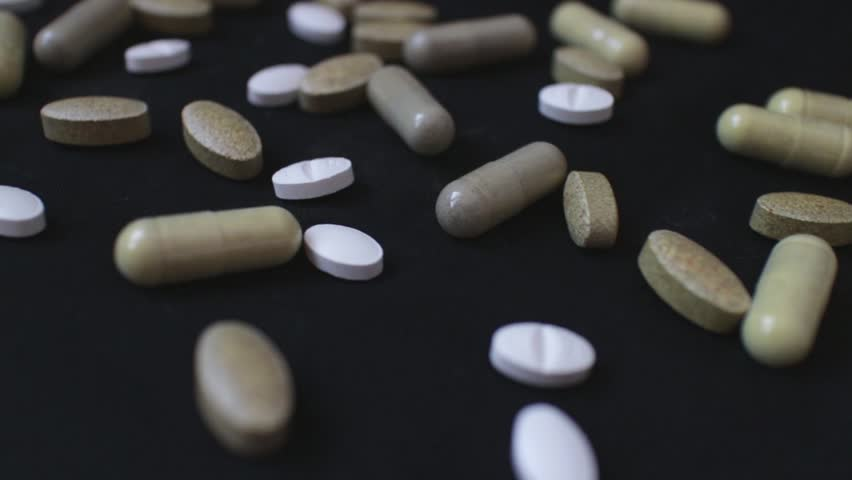
\includegraphics[height=\paperheight]{../img/capsule-pills.jpg}
    }
    \maketitle
  }

  \begin{frame}{Outline}
    \tableofcontents
  \end{frame}

%%%%%%%%%%%%%%%%%%%%%%%%%%%%%%%%%%%%%%%%%%%%%%%%%%%%%%%%%%%%%%%%%%%%%%%%%%%%%%%%

  \section{The Alpha* Timeline}

%%%%%%%%%%%%%%%%%%%%%%%%%%%%%%%%%%%%%%%%%%%%%%%%%%%%%%%%%%%%%%%%%%%%%%%%%%%%%%%%

  \section{AlphaGo}

%%%%%%%%%%%%%%%%%%%%%%%%%%%%%%%%%%%%%%%%%%%%%%%%%%%%%%%%%%%%%%%%%%%%%%%%%%%%%%%%

  \section{AlphaGo Zero (AG0)}

%%%%%%%%%%%%%%%%%%%%%%%%%%%%%%%%%%%%%%%%%%%%%%%%%%%%%%%%%%%%%%%%%%%%%%%%%%%%%%%%

  \section{AlphaZero}

%%%%%%%%%%%%%%%%%%%%%%%%%%%%%%%%%%%%%%%%%%%%%%%%%%%%%%%%%%%%%%%%%%%%%%%%%%%%%%%%

  \section{Conclusion}

  \begin{frame}[standout]
    \begin{center}
      Thank you!

      Questions?
    \end{center}
  \end{frame}

%%%%%%%%%%%%%%%%%%%%%%%%%%%%%%%%%%%%%%%%%%%%%%%%%%%%%%%%%%%%%%%%%%%%%%%%%%%%%%%%

  \appendix
  \begin{frame}[standout]
    Backup Slides
  \end{frame}

  % TODO display (I), (II) instead of i, ii
  \begin{frame}[allowframebreaks]{Further Reading}
    \tiny
    Artificial Intelligence:
    \begin{itemize}
      \item \textbf{Artificial Intelligence course at MIT} \url{http://ocw.mit.edu/courses/electrical-engineering-and-computer-science/6-034-artificial-intelligence-fall-2010/index.htm}
      \item \textbf{Introduction to Artificial Intelligence at Udacity} \url{https://www.udacity.com/course/intro-to-artificial-intelligence--cs271}
      \item \textbf{General Game Playing course} \url{https://www.coursera.org/course/ggp}
      \item \textbf{Singularity} \url{http://waitbutwhy.com/2015/01/artificial-intelligence-revolution-1.html} + Part 2
      \item \textbf{The Singularity Is Near} (\cite{Kurzweil2005singularity})
    \end{itemize}

    Machine Learning:
    \begin{itemize}
      \item \textbf{Machine Learning course} \url{https://youtu.be/hPKJBXkyTK://www.coursera.org/learn/machine-learning/}
      \item \textbf{Reinforcement Learning} \url{http://reinforcementlearning.ai-depot.com/}
      \item \textbf{Deep Learning} (\cite{Lecun2015deep})
      \item \textbf{Deep Learning course} \url{https://www.udacity.com/course/deep-learning--ud730}
      \item \textbf{Two Minute Papers} \url{https://www.youtube.com/user/keeroyz}
      \item \textbf{Applications of Deep Learning} \url{https://youtu.be/hPKJBXkyTKM}
    \end{itemize}

    Neuroscience:
    \begin{itemize}
      \item \url{http://www.brainfacts.org/}
    \end{itemize}
  \end{frame}

  \begin{frame}[allowframebreaks]{References}
    \tiny
    \printbibliography[heading=none]
  \end{frame}

\end{document}
